\begin{figure}
    \centering
    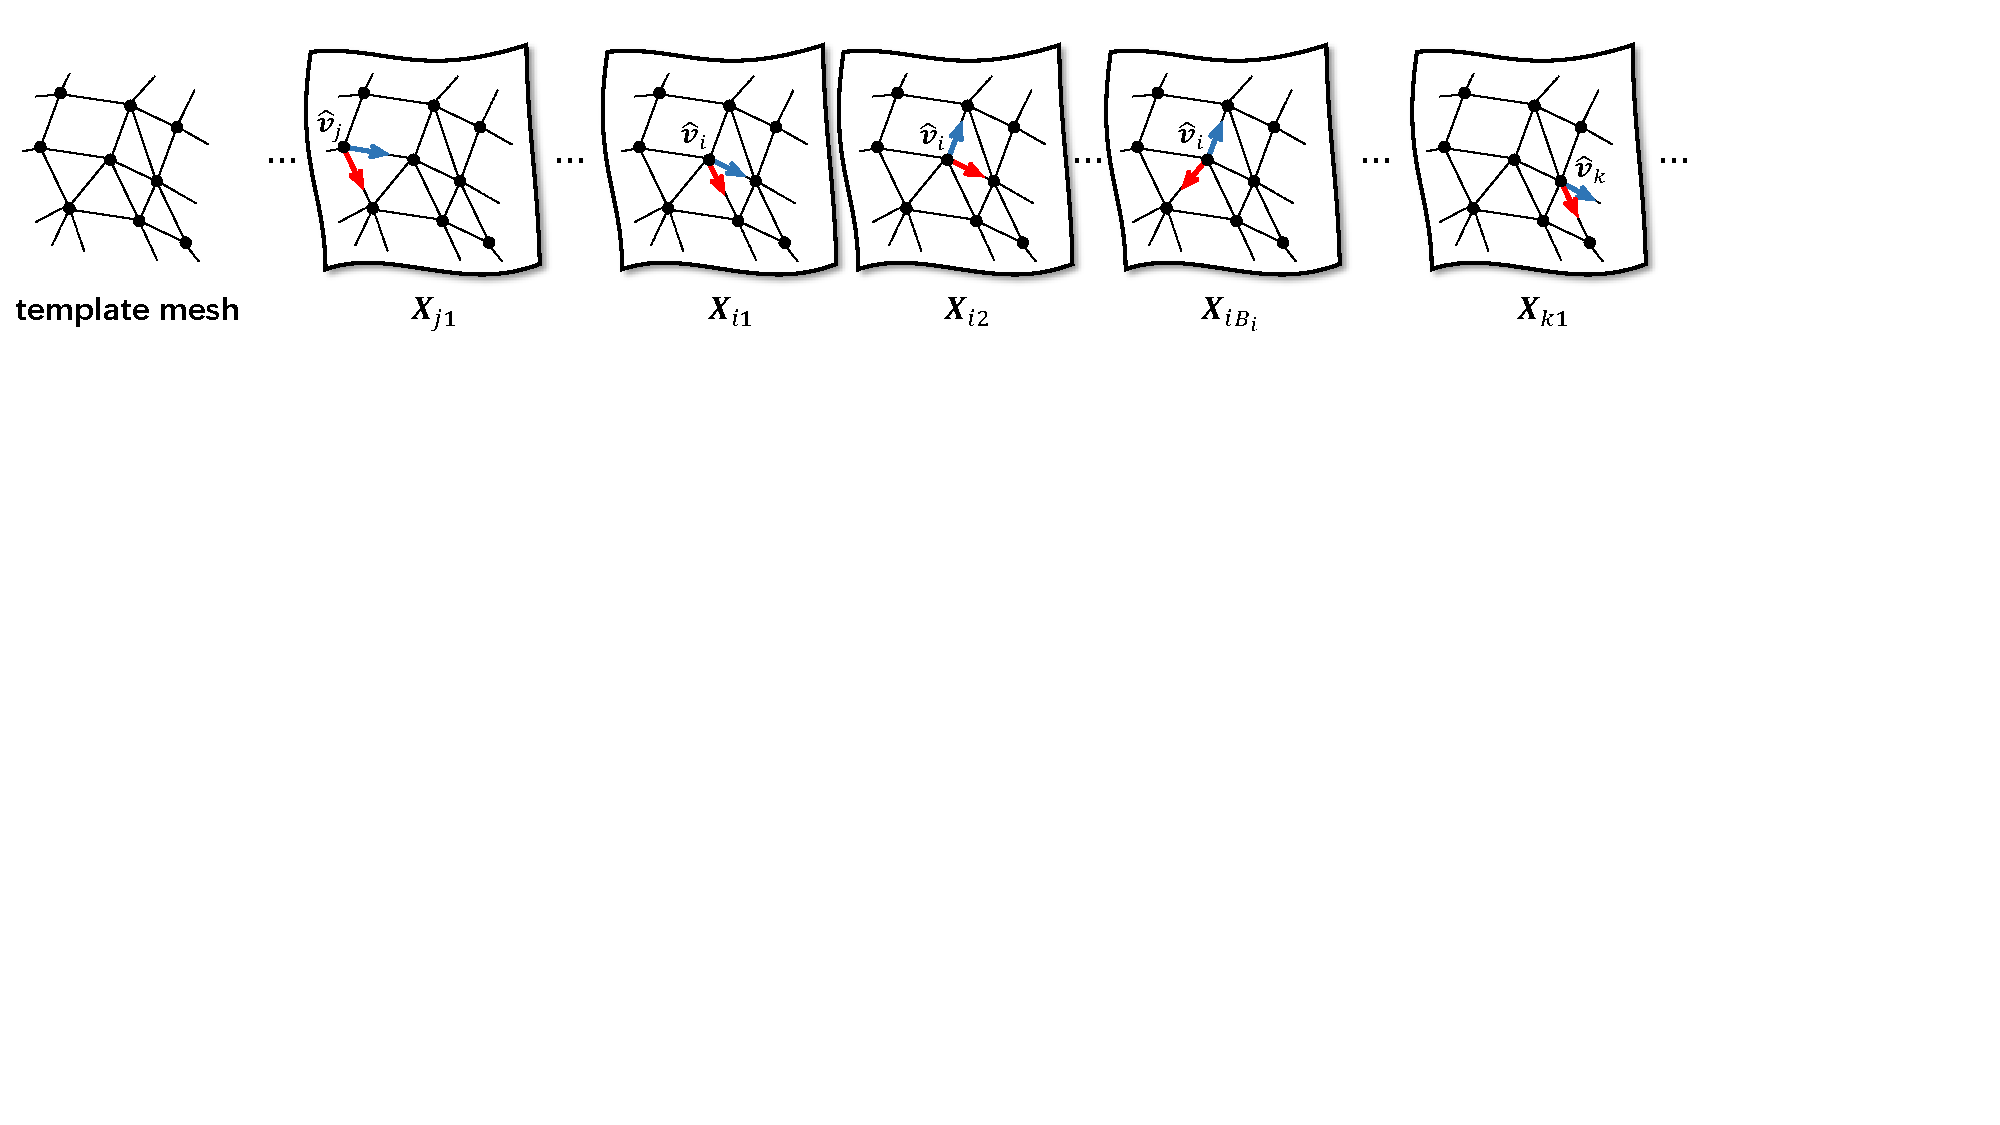
\includegraphics[width=1\linewidth]{chapter3/tex/figures/active_model_K_sum.pdf}
    \caption{\small The multiple skewed coordinate systems build on different vertex and pairs of neighbors.}
    % {\bf The template mesh and the non-rigid coordinate systems for parameterization. Each coordinate system $X$ is build on a vertex and a unique pair of neighbors. An energy function is defined for every $X$ to measure the mesh distortion locally at a certain orientation. The origins of $X$s are at the Cartesian origin. We attach it to vertices for visualization clarity} }
    \label{ch3:fig:sum_coords}
\end{figure}